\chapter{Implementação de Software para Controle de Sistemas Robóticos}
A implementação dos algoritmos de controle detalhados nos capítulos anteriores for feita como extensão ao software RobotGUI desenvolvido pela equipe do LEAD-GSCAR \citep{nunes2013doris}.

Proporciona uma infraestrutura para carregar componentes modulares de software para robôs, juntamente com classes altamente reutilizáveis. Esses sistema permite inicializar módulos de software com uma interface gráfica associada, de modo a interagir com eles. Por exemplo, ao iniciar componente que obtêm dados de um sensor, é iniciada na interface gráfica uma \textit{Tool} que permite visualizar os dados e configurar parâmetros. Essa conexão é dinâmica, permitindo que componentes sejam iniciados de forma independente e até mesmo em momentos diferentes.  


\section{Ferramentas}
Os seguintes softwares e \textit{frameworks} foram utilizados:

\begin{itemize}
\item Linux (Ubuntu 14.04/16.04) como Sistema Operacional
\item C++ como linguagem de programação
\item Robot Operating System \citep{quigley2009ros} como \textit{framework} principal utilizado pelo RobotGUI, fornecendo comunicação entre nós através de mensagens e serviços. Será descrito mais detalhadamente na próxima seção.
\item Qt \citep{qtcompany} como \textit{framework} para elaboração da interface gráfica. 
\item Julia Language como linguagem auxiliar na elaboração de algoritmos de controle modificáveis em tempo de execução
\end{itemize}

\section{Robot Operating System (ROS)}
Escrever software para robôs tem se tornado particularmente difícil conforme a escala e o escopo dos projetos de robótica continua a crescer. Robôs podem ser de diferentes tipos e ter hardware completamente distinto, o que torna a reutilização de código difícil. Além disso, a quantidade de código necessário para um projeto de robótica pode ser intimidadora, indo desde software a nível de \textit{driver} até percepção e raciocínio, por exemplo. Como o nível de conhecimento e experiência necessário é maior do que um pesquisador sozinho pode ter, arquiteturas de software para robótica devem suportar integração. 

Em \citep{quigley2009ros} é descrito o framework ROS, que busca enfrentar esses desafios. A enfase dada a projetos integrados de grande escala é útil em uma variedade de aspectos conforme sistemas robóticos tornam-se mais complexos. Os objetivos de projeto do ROS podem ser resumidos como: 
\begin{itemize}
\item \textbf{Peer-to-peer ou ponto-a-ponto:} Um sistema construído utilizando ROS consiste de um conjunto de processos, potencialmente em diferentes máquinas hospedeiras e conectados entre si em uma topologia ponto-a-ponto. Tipicamente existe um ou mais computadores embarcados conectados via \textit{ethernet}, que se comunicam via rede \textit{wireless} com máquinas com maior poder computacional, capazes de realizar tarefas como visão computacional e reconhecimento de fala. 

\item \textbf{Multi-Linguagem:} Muitos possuem preferência em relação a determinadas linguagens de programação devido a fatores como tempo para escrita do código, facilidade de \textit{debugging}, sintaxe ou eficiência de execução. ROS suporta as linguagens C++, Python, Octave e LISP. O ROS faz uma especificação a nível de mensagens. A configuração e negociação da conexão ponto a ponto ocorre através de XML-RPC \footnote{RPC, do inglês, Remote Procedure Call é um termo da computação distribuída usado para quando um programa de computador causa a execução de um procedimento (subrotina) em outro espaço de endereçamento (outro computador na mesma rede).}, para o qual existem implementações na maioria das linguagens.   

É utilizada uma linguagem de definição de interface (IDL) que descreve as mensagens enviadas entre módulos. Código nativo de cada linguagem é gerado a partir dessas mensagens. 


\item \textbf{Baseado em ferramentas:} Para dar conta da complexidade do ROS seus desenvolvedores optaram por um design \textit{microkernel}, em contraste a um design monolítico. Essas ferramentas cumprem tarefas como navegar pela árvore de código fonte, configurar parâmetros, visualizar a topologia dos nós, publicar e exibir mensagens, entre outros.

\item \textbf{Fino:} Muitos projetos de software para robótica possuem drivers e algoritmos que poderiam ser reutilizados mas estão altamente "amarrados" ao software em questão, de modo que é difícil extrair e reutilizar essas funcionalidades.

No ROS, encoraja-se a encapsular todos os drivers e algoritmos em bibliotecas independentes. 


\item \textbf{Gratuito e código aberto:} Todo o código fonte do ROS está disponível publicamente. Isso é critico para facilitar a descoberta e correção de erros. É distribuído sob os termos da licença BSD.  

\end{itemize}

\subsection{Conceitos Básicos}
Esta seção se baseia em \citep{ros_concepts} e busca detalhar conceitos do funcionamento e arquitetura do ROS necessários ao entendimento do software desenvolvido nesse trabalho. 

%\subsection{Nível de Sistema de Arquivos}

\subsection{Nível de Grafo de Computação}
Os conceitos a nível de grafo de computação descrevem elementos da rede ponto-a-ponto de processos ROS que estão em execução juntos. Esses elementos são descritos abaixo com seus nomes mantidos em inglês por fidelidade ao original.
\begin{description}
\item[Nodes:] Nós são processos que executam algum tipo de computação. ROS foi projetado para ser modular, assim um sistema de controle de um robô geralmente tem múltiplos nós. 

\item[Master:] Devido a topologia ponto-a-ponto é necessário um mecanismo de busca que os processos se encontrem. O mestre é um servidor de nomes, ou seja, provê registro e busca de nomes.

\item[Parameter Server:] O servidor de parâmetros permite que dados sejam armazenados em uma localização central. Faz parte do \textit{Master}.

\item[Messages:] Nós comunicam entre si passando mensagens. Uma mensagem consiste apenas de uma estrutura de dados. Mensagens suportam tipos primitivos, \textit{arrays} de tipos primitivos ou outras estruturas aninhadas. 

\item[Topics:] Um nó envia uma mensagem publicando a um dado tópico. O nome do tópico é utilizado para identificar o conteúdo da mensagem. Um outro nó que esteja interessado nesse conteúdo pode subscrever ao tópico. Podem existir múltiplos \textit{publishers} e \textit{subscribers} para o mesmo tópico e um nó pode publicar e/ou subscrever a múltiplos tópicos. 

\item[Services:] Em muitos casos é necessário ter um mecanismo de comunicação um para um de modo a lidar com interações do tipo pedido/resposta. Isso é feito através de serviços, que são definidos por um par de estruturas como as mensagens, uma para o pedido e outra para a resposta. Um nó oferece um serviço sob um nome e um cliente utiliza o serviço mandando um mensagem de pedido e esperando uma resposta. As bibliotecas do ROS apresentam essa interação na forma de um chamada de procedimento remoto (RPC).

\item[Bags:] Bags são um formato para salvar e reproduzir dados de mensagens de ROS ao longo do tempo. São úteis para salvar dados de sensores, por exemplo, que são difíceis de coletar mas necessários para o desenvolvimento de algoritmos. 
\end{description}

O \textit{ROS Master} funciona como um servidor de nomes. Ele armazena informação de registro para os nós, que se comunicam com o Master para reportar sua informação de registro. Conforme os nós se comunicam com o \textit{Master}, eles podem receber informação sobre outros nós registrados e fazer as conexões apropriadas. \textit{Master} 

Nós conectam-se diretamente a outros nós, o \textit{Master} somente fornece informação de busca, como um servidor DNS. Nós que subscrevem a um tópico vão solicitar conexão aos nós que publicam naquele tópico e irão estabelecer a conexão de acordo com um protocolo de conexão concordado. O protocolo mais comum é chamado de TCPROS, que utiliza sockets TCP/IP padrão.

Essa arquitetura permite uma operação desacoplada. Nós, tópicos, serviços e parâmetros possuem nomes. Por meio deles sistemas maiores e mais complexos podem ser construídos. É possível remapear nomes, de modo que um programa compilado  pode ser reconfigurado para operar com uma topologia diferente. 

%\subsection{Nível de Comunidade}

\subsection{Nodelets}
O pacote Nodelet foi projetado de forma a permitir a execução de múltiplos algoritmos no mesmo processo sem \textit{overhead} \footnote{Processamento ou armazenamento em excesso, seja de tempo de computação, de memória, de largura de banda ou qualquer outro recurso que seja gasto para executar uma determinada tarefa.}, devido a comunicação entre nós (não há custo de cópia). Esse pacote fornece a classe Nodelet, utilizada para implementar um nodelet e a classe nodelet::Loader utilizada para instanciar nodelets. 

\section{Arquitetura do RobotGUI}

Primeiramente define-se como computador base aquele que será utilizado pelo operador para controlar e visualizar dados do robô. Define-se computador embarcado, ou do robô, o computador especificação PCIe/104, descrito no capítulo \ref{chap:descricao_hard}. O software executa nós diferentes no robô e na base.

A arquitetura do RobotGUI baseia-se nos seguintes conceitos principais \citep{nunes2013doris}:

\begin{itemize}
\item \textbf{Components}: Lidam com a comunicação e processam dados no Computador Base. São essencialmente \textit{Nodelets} de ROS, podendo utilizar funcionalidades como comunicação através de mensagens e serviços, utilizar parâmetros e bibliotecas de ROS. Permitem maior modularidade pois componentes podem ser inicializados independentemente do \textit{RobotGUI}.

\item \textbf{Tools:} São elementos gráficos da interface para o usuário. São utilizadas para interagir com o robô e visualizar informação. São criadas como \textit{plugins} para o ROS \textit{pluginlib} e independetes de qualquer biblioteca do ROS.

\item \textbf{Devices:} São \textit{Components} utilizados para representar um dispositivo do robô. Utilizam o mecanismo de \textit{Item} e \textit{Variable} e se conectam a \textit{Tools} padrão fornecidas pelo RobotGUI, que são \textit{DataTable}, \textit{Device Management} e \textit{Plotter}. 

\item \textbf{Item e Variable:} \textit{Variables} contém valores de interesse, sempre guardando um valor desejado e um valor real. Por exemplo em uma variável controlada o valor desejado será a referência dada pelo operador e o valor real é obtido de algum sensor. Para mostrar esses valores na interface utiliza-se \textit{Items}. Uma \textit{Variable} pode estar associada a diversos \textit{Items}, de forma que através desse mecanismo o valor exibido em todos eles é atualizado. 

\item \textbf{Interação entre Compontents e Tools:} Tools e Components podem se conectar, quando isso ocorre eles interagem entre si a nível de "ponteiro para objeto". Essa conexão permite que o desenvolvimento da interface através do \textit{Qt} seja quase que independente do desenvolvimento do código que lida com hardware, lógica e comunicação. Essas classes disponibilizam uma estrutura para conectar \textit{Components} e \textit{Tools} de tal forma que quano um \textit{Component} é iniciado ele busca por \textit{Tools} associadas a ele que estejam em execução e vice versa. Quando um \textit{Component} é 

\item \textbf{RobotGUI:} É uma GUI \footnote{Guided User Interface} em nó de ROS. Permite que múltiplas janelas sejam criadas. O usuário pode decidir o que é exibido. Ao clicar nos \textit{toolbuttons}, uma janela referente a \textit{Tool} aparece. Essa janela pode ser encaixada na janela principal. O RobotGUI executa \textit{roslaunch}'s, nós incluídos pelo \textit{roslaunch} em questão podem ser \textit{Components}. 

\item \textbf{NodeletManager e RobotGUI:} o RobotGUI é um Nodelet Manager com pequenas modificações. Um NodeletManager utiliza a classe nodelet::Loader para instanciar nodelets. Utilizando uma versão modificada dessa classe é possível verificar se um Nodelet a ser carregado é um \textit{Component}. Se esse for o caso, a \textit{Tool} correspondente será carregada e as conexões são feitas. Quando um componente é descarregado, a conexão com as \textit{Tools} associadas a ele é encerrada.
\end{itemize}


%\href{run:pf-luisgustavo-v004.pdf}{Click to execute}% 

\subsection{Topologia}

No diagrama da figura \ref{fig:ros_nodes} são mostados os nós executados pelo programa para utilizar o manipulador e como se comunicam. Elipses representam Nodes, elipses tracejadas representam Nodelets e retângulos representam tópicos. Os retângulos que contém outros elementos representam os pacotes aos quais aqueles nós pertencem. Quando as setas saem de um nó, representam que o nó publica informação em um tópico, e quando chegam, representam que ele subscreve ao tópico em questão. As linhas pontilhadas representam que os \textit{Nodelets} aos quais elas estão conectadas são executadas pelo \textit{Node} na outra extremidade. Neste diagrama, são omitidos os tópicos de configuração de parâmetros.

\begin{figure}[!h]
  \centering
  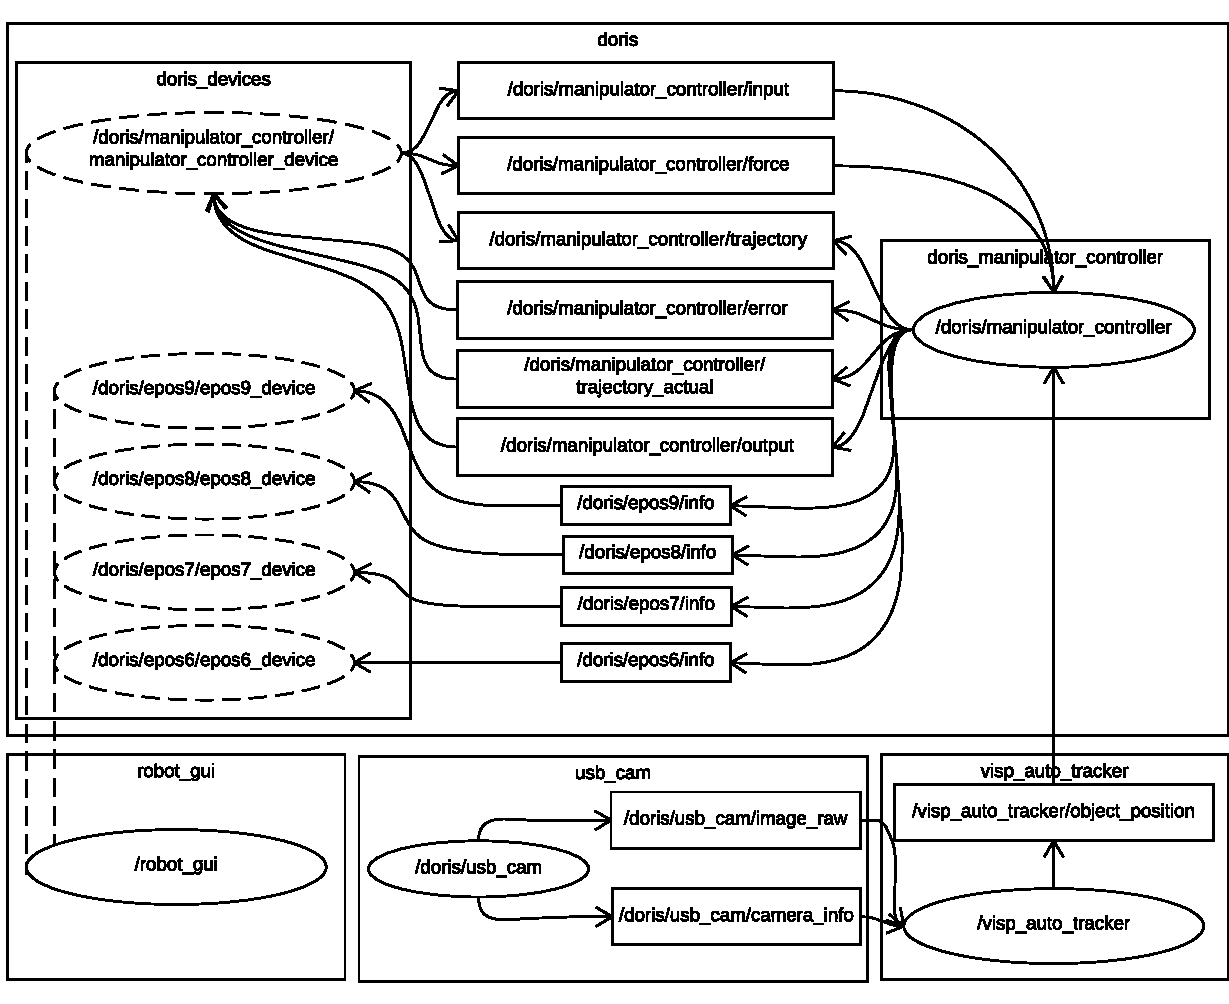
\includegraphics[width=\linewidth]{./img/node_diagram}
  \caption{ROS Nodes}
  \label{fig:ros_nodes}
\end{figure}

Os \textit{ROS Nodes} \verb|manipulator_controller| e \verb|usb_cam| são executados no computador embarcado. Os nós \textit{Nodes} \verb|robot_gui|, \verb|visp_auto_tracker| são executados no computador base. Os \textit{Nodelets} \verb|manipulator_controller_device| e os \verb|eposX_device| são carregados pelo \verb|robot_gui|, que é um \textit{Nodelet Manager}. 

\subsection{ManipulatorControllerDevice}

A classe ManipulatorControllerDevice deriva de Device. Possui as \textit{Variables} mostradas na tabela \ref{tab:variables}. Essa classe faz a interface entre \textit{Tools} e os tópicos de ROS. Ao receber uma mensagem de ROS, um \textit{callback} referente ao tópico em questão é executado atualizando a variável associada àquela informação. A atualização da variável resulta na atualização do \textit{Item}.

\begin{table}[h!]
\centering
\caption{\textit{Variables} do \textit{ManipulatorControllerDevice}}
\label{tab:variables}
\begin{tabular}{rl} \hline
Variable & Descrição \\ \hline
\verb|coast| & 				Comando de parar o controle das juntas. \\
\verb|home| &  				Comando de ir para posição inicial. \\
\verb|record|& 				Comando de iniciar a gravação de Logs.\\
\verb|zeroForce|& 			Comando de \textit{reset} do sensor de Força.\\
\verb|ktGain|&				Ganho $K_t$ para rastreamento de trajetória. \\
\verb|kjGain|&				Ganho $K_j$ para controle no espaço das juntas.\\
\verb|kvGain|&				Ganho $K_v$ para controle por servo visão.\\
\verb|kfGain|&				Ganho $K_f$ para controle de força.\\
\verb|pidParameters|&		Parâmetros do controlador PID para controle de força.\\
\verb|x|&					Vetor $\bm{x_e}$ conforme definido em \ref{eq:operational_space}.\\				
\verb|error|&				Erro conforme definido em \ref{eq:error_pf}.\\
\verb|output|&				Saída $\bm{u}$ do controlador.\\
\verb|controlMode|&			Modo de controle selecionado (detalhes em \ref{sec:ctrlmodes}). \\
\verb|individualMode|&		Modo de controle individual selecionado (detalhes em \ref{sec:ctrlmodes}).\\
\verb|positionValue|&		Valor de posição cartesiana (refererência/medido). \\
\verb|forceValue|&			Valor de força (refererência/medido).\\
\verb|individualValue|&		Valores para controle individual.  \\
\verb|openLoopVelocityEfct|&Valores para malha aberta de velocidade em $E_e$. \\
\verb|openLoopVelocityBase|&Valores para malha aberta de velocidade em $E_b$. \\
\verb|qValue|&				Valor de $\bm{q}_d$ e $\bm{q}$ para controle no espaço das juntas.	\\
\verb|trajectory|&			Trajetória na forma de código em \textit{Julia Language}\\
\hline
\end{tabular}
\end{table}

\subsection{DorisManipulatorController}

A classe DorisManipulatorController deriva da classe Controller, que implementa a estrutura necessária para a criação de um controlador. Ela permite que o controle seja executado com um período fixo, em uma \textit{thread} interna, ou que o ciclo de controle seja executado por uma chamada externa. Nesse caso é utilizada a primeira opção. Possui a funcionalidade de receber entradas de múltiplas fontes. Por exemplo, o manipulador pode ser controlado por uma janela na interface e por um \textit{joystick}. O Controller está pronto para lidar com isso, quando uma fonte fica inativa, outra é capaz de controlar. 

A entrada do Controller é uma mensagem de controle com a seguinte forma.

\begin{lstlisting}[caption=Control.msg]
uint8 originId
uint8[] modes
float64[] data
\end{lstlisting}

O primeiro campo identifica a fonte da mensagem. O segundo é um \textit{array} de modos de cotrole. O primeiro elemento é o modo principal, enquando os demais, se existirem, são submodos. O terceiro elemento \verb|data| é um \textit{array} de elementos em ponto flutuante que contém a referência de controle. Pode ser vazio caso o modo de controle seja autônomo ou receba dados de outra fonte.

\begin{figure}[!h]
  \centering
  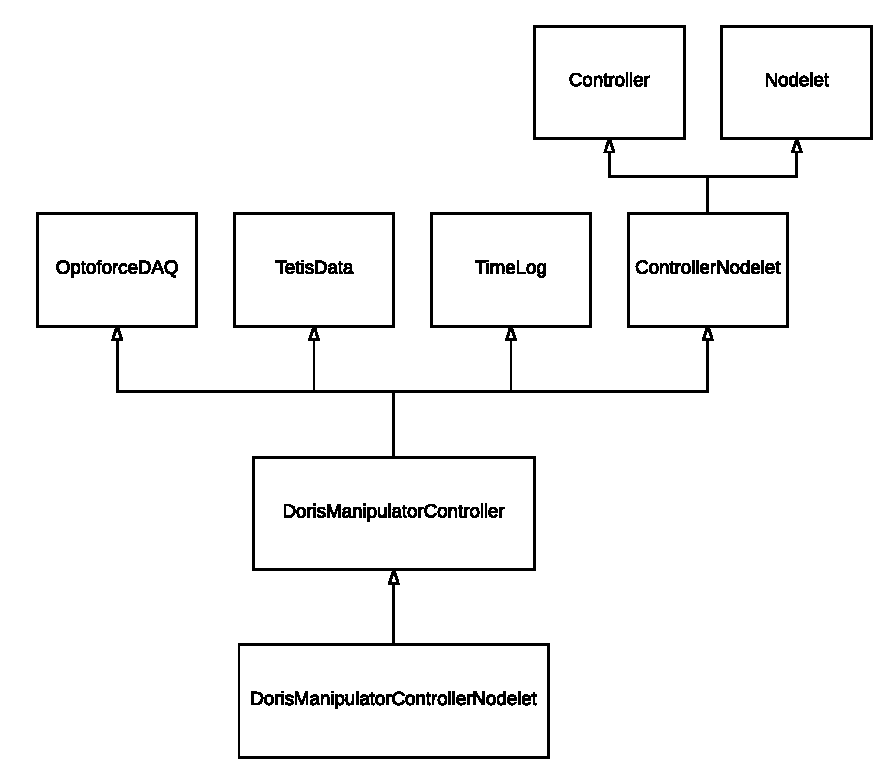
\includegraphics[width=0.9\linewidth]{./img/class_diagram}
  \caption{Diagrama de classes para o DorisManipulatorController}
  \label{fig:classes}
\end{figure}

Seguindo os princípios do ROS, busca-se separar em classes a interação com ROS de algoritmos de controle. As classes com terminação em \textit{Nodelet} herdam dessa classe e, portanto, implementam toda a comunicação (mensagens, serviços, etc.). A classe DorisManipulatorController implementa o ciclo de controle, chaveamento entre modos de controle, assim como os algoritmos de controle. OptoforceDAQ é uma classe utilizada para fazer a aquisição de dados do sensor de força Optoforce descrito na seção \ref{sec:optoforce}. A classe TetisData encapsula dados específicos do manipulador TETIS como dimensões dos elos e ângulos de juntas. A classe TimeLog é uma utilidade para salvar dados e gerar logs de forma automatizada. 

\subsection{Modos de controle} \label{sec:ctrlmodes}

A classe DorisManipulatorController implementa os modos de controle descritos na tabela . 


\begin{table}[h!]
\centering
\caption{\textit{Variables} do \textit{ManipulatorControllerDevice}}
\label{tab:variables}
\begin{tabular}{rl} \hline
Modo de controle      	& Descrição \\ \hline
\verb|NotControlled|  	& Nenhum sinal de controle é enviado ao manipulador.\\
Brake 				  	& Sinal de controle $u = 0$. \\
OperationalSpace 	  	& Implementa o controle descrito em \ref{sec:openloopbase}. \\
Vision 				  	& Implementa o controle descrito em \ref{sec:servo_vision}. \\
VelocityEfct 			& Implementa o controle descrito em \ref{sec:openloopefct}. \\
VelocityBase 			& Implementa o controle descrito em \ref{sec:openloopbase}. \\
PplusFF 				& Implementa o controle descrito em \ref{sec:pplusf}. \\
Force 					& Implementa o controle descrito em \ref{sec:forca_approach}. \\
JointSpace 				& Implementa o controle descrito em \ref{joint_space}. \\
Individual 				& Implementa o controle individual de juntas por gerador de função. \\
MasterSlave				& Estrutura preparada para integração com o Sensable\circledR Phantom Omni. \\
\hline
\end{tabular}
\end{table}


\begin{itemize}
	\item NotControlledI
	\item BrakeI
	\item Constant
	\item Square
	\item Pulse
	\item Sine
	\item JointSpaceMS
	\item VelocityToolMS
\end{itemize}

\subsection{DorisManipulatorTool}
Para interagir com o manipulador é utilizada a \textit{Tool} chamada DorisManipulatorTool. Ela permite alternar entre os modos de controle listados acima, ajustar parâmetros e ganhos dos controladores e alterar referências. A imagem \ref{fig:screenshot1} mostra a interface com DorisManipulatorTool a direita,  Plotter no canto esquerdo superior, e DeviceManagement no canto esquerdo inferior.
 
\begin{figure}[!h]
  \centering
  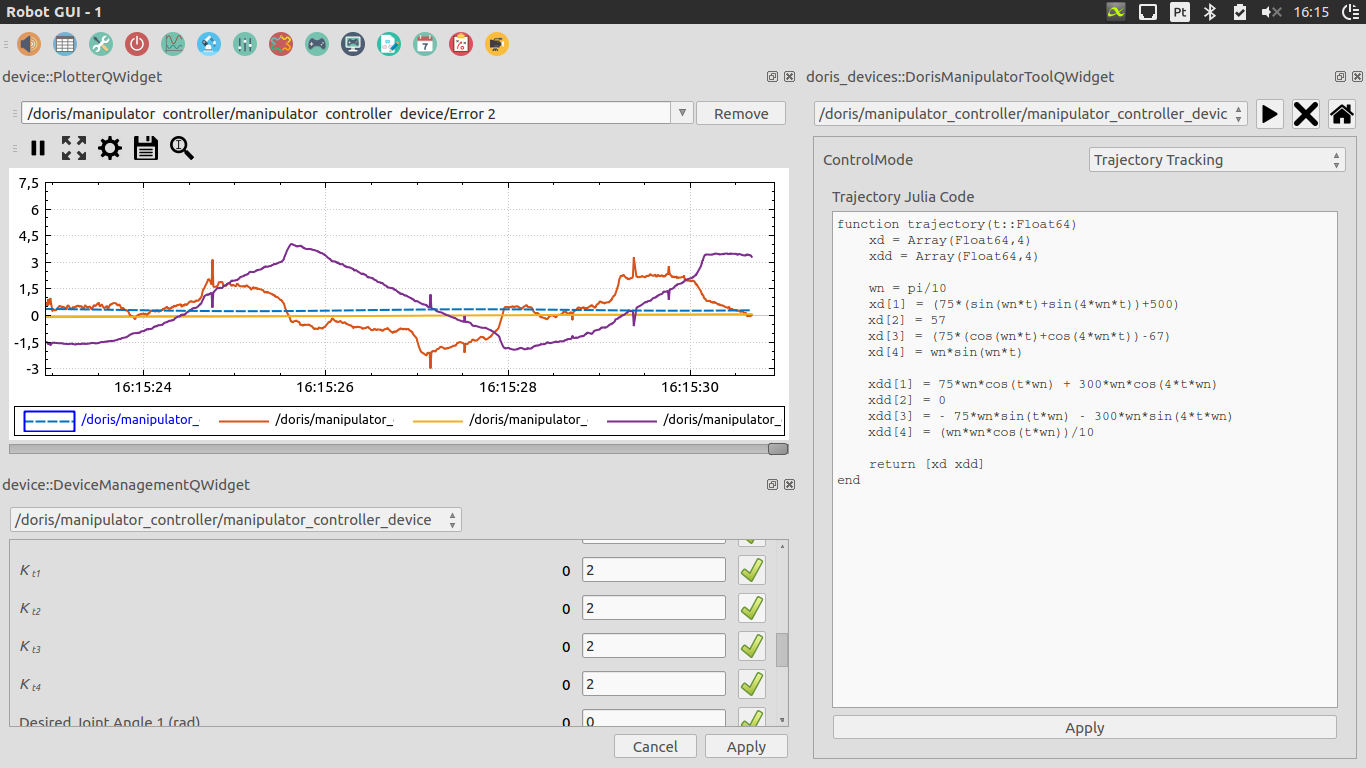
\includegraphics[width=\linewidth]{./img/screenshot/sc1.png}
  \caption{RobotGUI com três \textit{Tools}: DorisManipulatorTool, Plotter e DeviceManagement}
  \label{fig:screenshot1}
\end{figure}


\begin{figure}[!h]
  \centering
  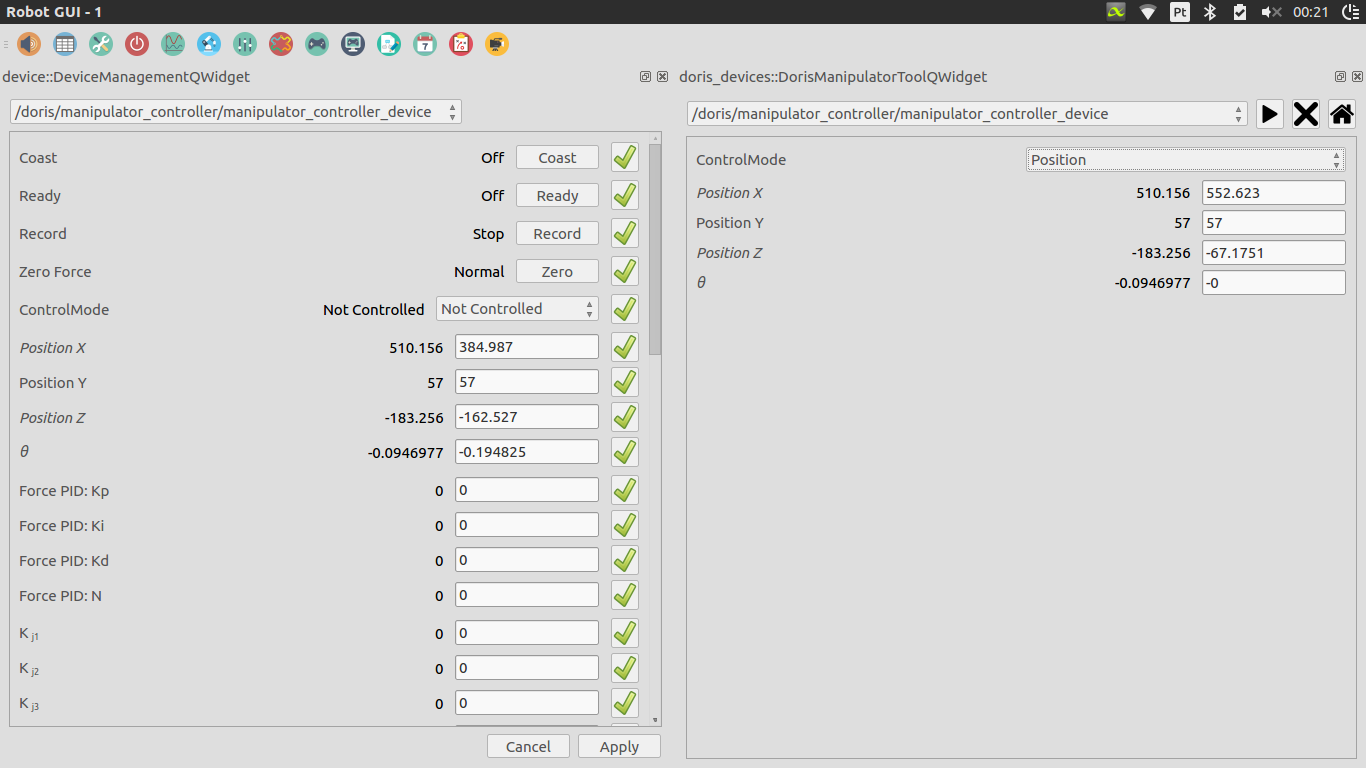
\includegraphics[width=\linewidth]{./img/screenshot/sc2.png}
  \caption{RobotGUI com DorisManipulatorTool e DeviceManagement}
  \label{fig:screenshot2}
\end{figure}

\section{Julia Language}

\textit{Julia} é uma linguagem dinâmica de alto nível e alta performance, projetada para computação técnica. Possui uma sintaxe familiar para usuários de outras linguagens orientadas a computação científica. Dentre as funcionalidades que a linguagem proporciona, destacam-se para a aplicação neste projeto:

\begin{itemize}
\item Boa performance, aproximando-se de linguagens estaticamente compiladas como C.
\item Tipagem dinâmca: tipos podem ser utilizados para documentação e otimização.
\item Compilador \textit{just-in-time} \footnote{Compilação just-in-time (JIT) refere-se a compilação feita no momento de execução do programa, com contraste com compilação anterior a execução.} de alta performance.
\item Gratuito e código aberto (Licença MIT).
\item Possibilidade de integrar Julia a projetos C/C++.
\end{itemize}

A compilação \textit{just-in-time} é baseada no projeto LLVM \citep{llvmorg,lattner2004llvm}, que consiste em uma coleção de tecnologias e ferramentas compilação modulares e reutilizáveis. O uso dessas tecnologias, juntamente com a forma como a linguagem foi projetada permite em muitos casos ela tenha uma performance comparável com a linguagem C e ao mesmo tempo ter uma sintaxe comparativamente simples.

Portanto, a linguagem Julia mostrou-se uma opção interessante e mais dinâmica para a implementação de controle no software de controle para o TETIS, que requer desempenho mas pode se beneficiar de uma linguagem dinâmica. Uma prova de conceito foi feita para o para a configuração das equações da trajetória a ser rastreada. Na interface uma janela permite a escrita de equações na forma de uma função Julia. Ao aplicar as alterações esse código é enviado para o computador embarcado através do ROS. O programa principal, em C++, chama a API em C do Julia e compila essa função no momento da primeira execução.

Dessa forma a trajetória pode ser alterada em tempo de execução sem prejudicar a performance e sem necessitar acesso a dados externos constantemente. O código em \ref{lst:julia} mostra a trajetória de teste em \textit{Julia Language}.

\begin{lstlisting}[caption={trajectory.jl}\label{lst:julia}]
function trajectory(t::Float64)
	xd = Array(Float64,4)
	xdd = Array(Float64,4)

	wn = pi/10
	xd[1] = (75*(sin(wn*t)+sin(4*wn*t))+500)
    xd[2] = 57
    xd[3] = (75*(cos(wn*t)+cos(4*wn*t))-67)
    xd[4] = wn*sin(wn*t)

    xdd[1] = 75*wn*cos(t*wn) + 300*wn*cos(4*t*wn)
    xdd[2] = 0
    xdd[3] = - 75*wn*sin(t*wn) - 300*wn*sin(4*t*wn)
    xdd[4] = (wn*wn*cos(t*wn))/10
	
	return [xd xdd]
end
\end{lstlisting} 


